\subsection{Measurement Methodology}

\begin{figure}[!tb]
\centering
%%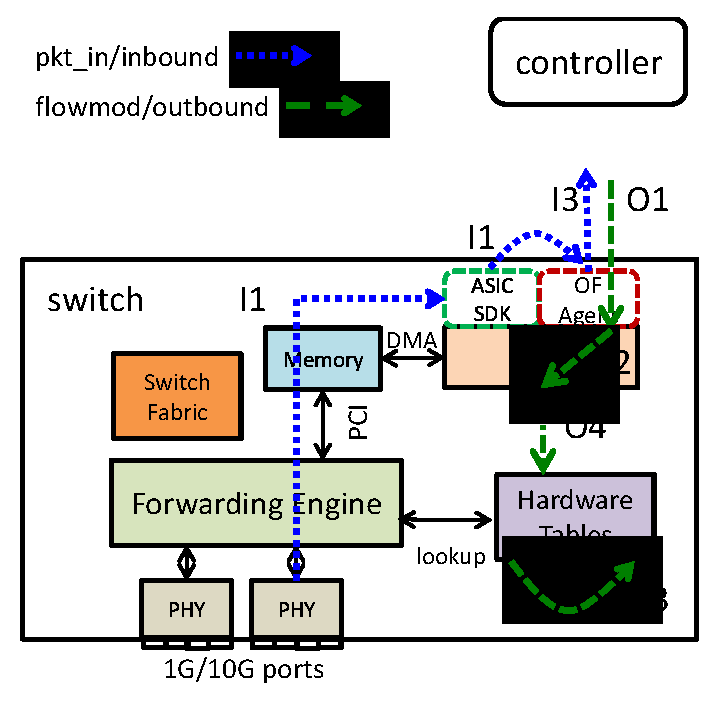
\epsfig{file=./figs/openflow_switch_illustrate.eps,width=0.4\textwidth} %%changed
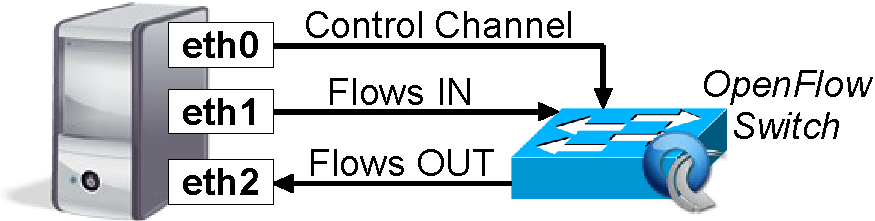
\includegraphics[width=0.7\columnwidth]{figs/experiment_setup.pdf}
\botcompactcaption{Measurement experiment setup. }\label{experiment_setup} 
%\marina{add pox controller and pkt capture points on the fig}
\end{figure}

\figref{experiment_setup} shows our measurement setup.
The host has one 1Gbps and two 10Gbps interfaces that are connected to the switch under test. 
The eth0 interface is connected to the control port of the switch, and an SDN
controller (POX for \Intel and \BroadcomOne, RYU for \BroadcomThree) running
on the host listens on this interface. 
%To ensure that the switch is not bypassed the eth1 and eth2 ports have different network name spaces. 
The propagation delay between switch and controller is
negligible (about 0.03ms). We use the controller to send a burst of OpenFlow 
\flowmod commands to the switch. For \Intel and \BroadcomOne, we
install/modify/delete rules in the single table supported by OpenFlow 1.0;
for \BroadcomThree, we use the highest numbered table, which supports
rules defined over any L2, L3, or L4 header fields.
%For \Intel and \BraodcomOne we issue the commands for the default openflow 1.0 table and for \BroadcomThree, we issue commands for the table with the largest number of matching fields (ACL table).
The host's eth1 and eth2 interfaces are connected to data ports on the
switch. We run pktgen~\cite{pktgen} in kernel space to generate traffic on
eth1 at a rate of 600-1000Mbps.

Prior work notes that accurate execution times for OpenFlow commands on
commercial switches can only be observed in the data plane~\cite{oflops}.
Thus, we craft our experiments to ensure the latency impact of various
factors can be measured directly from the data plane (at eth2 in
\figref{experiment_setup}), with the exception of \packetin generation
latency. We run \emph{libpcap} on our measurement host to accurately
timestamp the packet and rule processing events of each flow. We first log
the timestamps in memory, and when the experimental run is complete, the
results are dumped to disk and processed. We use the timestamp of the
first packet associated with a particular flow as the finish time of the
corresponding \flowmod command; more details are provided later in this
section.
%further details on our latency calculations
%are presented later in this section.
%Further details on scenario-specific issues are discussed below.
%Further details that depend on the specific issues we measure are
%presented in later sections.
%\aaron{After reading again, my issue with this paragraph is that it's not
%clear what is done to measure \packetin latency.}

%  Other details of the measurement methodology is
% customized to clearly delineate the inbound and outbound delay
% components and will be discussed in the relevant sections.

%%\marina{We need a table with specific details of the switch - Switch type, Processor RAM, Data plane capacity, Max Flow table size, hardware and software tables, support for prioity, statistics gathering support}
